\chapter{Risikomanagement}\label{ch:risikomanagement}
Um Unwissenheiten im Entwicklungsprozess zu minimieren, ist es ein essenzieller Schritt mögliche Risiken frühzeitig 
zu erkennen, die den Projektablauf entweder positiv als Chance oder negativ als Bedrohung beeinflussen können.
Durch die Identifikation und Bewertung dieser Risiken können Maßnahmen ergriffen werden, um die negativen
Einflüsse zu minimieren und die positiven Einflüsse zu maximieren. \\
\newline
In ~\autoref{tab:risk} ist ein Risikoregister zu finden, das für die Einordnung möglicher Risiken erstellt wird. 
In diesem Register wird eine erarbeitete Sammlung an Risiken aufgeführt mit einer zugehörigen Nummer sowie einer
Beschreibung zur näheren Erläuterung.
Jedes Risiko besitzt eine eigene Eintrittswahrscheinlichkeit in Prozent mit einer Auswirkungsanalyse in den Graden 
gering, mittel oder groß, die die Bedrohlichkeit beziehungsweise Möglichkeit des Risikos darstellt.
Die Kategorisierung der Risiken unterteilt sich in die zwei Aspekte Art und Typ des Risikos, wobei der Typ den Einfluss
in positiver oder negativer Form, also Chance oder Bedrohung darstellt.
Abschließend wird jedem Risiko eine Behandlung mit zugehöriger Beschreibung beigefügt, damit Unwissenheiten bei der 
Entwicklung beseitigt werden und der Abschluss des Projekts sichergestellt werden kann. \\
\newline
Zur optimalen Veranschaulichung werden alle Risiken des Registers in einer Risikomatrix dargestellt, die die
Eintrittswahrscheinlichkeit gegen die Auswirkung aufträgt.
So kann auf einen Blick ein Risiko mit zum Beispiel starker Bedrohlichkeit erkannt werden und die entsprechende 
Behandlung eingeleitet werden. \\
\begin{figure}[h]
    \centering
    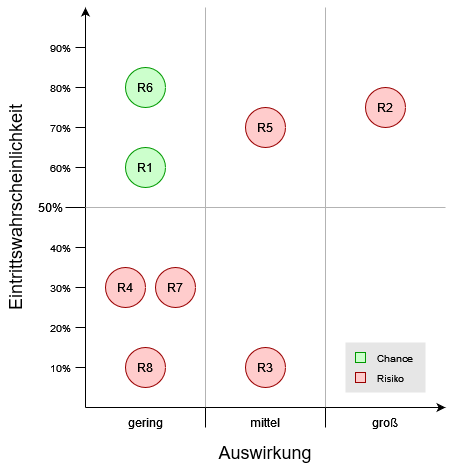
\includegraphics[width=0.5\linewidth]{../bilder/risk}
    \vspace{0.05cm}
    \caption{Risikomatrix}
    \label{fig:risk}
\end{figure}